\documentclass[]{article}
\usepackage{lmodern}
\usepackage{amssymb,amsmath}
\usepackage{ifxetex,ifluatex}
\usepackage{fixltx2e} % provides \textsubscript
\ifnum 0\ifxetex 1\fi\ifluatex 1\fi=0 % if pdftex
  \usepackage[T1]{fontenc}
  \usepackage[utf8]{inputenc}
\else % if luatex or xelatex
  \ifxetex
    \usepackage{mathspec}
  \else
    \usepackage{fontspec}
  \fi
  \defaultfontfeatures{Ligatures=TeX,Scale=MatchLowercase}
\fi
% use upquote if available, for straight quotes in verbatim environments
\IfFileExists{upquote.sty}{\usepackage{upquote}}{}
% use microtype if available
\IfFileExists{microtype.sty}{%
\usepackage{microtype}
\UseMicrotypeSet[protrusion]{basicmath} % disable protrusion for tt fonts
}{}
\usepackage[margin=1in]{geometry}
\usepackage{hyperref}
\hypersetup{unicode=true,
            pdftitle={Introduction to the R Programming Language},
            pdfauthor={Connor Hurd},
            pdfborder={0 0 0},
            breaklinks=true}
\urlstyle{same}  % don't use monospace font for urls
\usepackage{graphicx,grffile}
\makeatletter
\def\maxwidth{\ifdim\Gin@nat@width>\linewidth\linewidth\else\Gin@nat@width\fi}
\def\maxheight{\ifdim\Gin@nat@height>\textheight\textheight\else\Gin@nat@height\fi}
\makeatother
% Scale images if necessary, so that they will not overflow the page
% margins by default, and it is still possible to overwrite the defaults
% using explicit options in \includegraphics[width, height, ...]{}
\setkeys{Gin}{width=\maxwidth,height=\maxheight,keepaspectratio}
\IfFileExists{parskip.sty}{%
\usepackage{parskip}
}{% else
\setlength{\parindent}{0pt}
\setlength{\parskip}{6pt plus 2pt minus 1pt}
}
\setlength{\emergencystretch}{3em}  % prevent overfull lines
\providecommand{\tightlist}{%
  \setlength{\itemsep}{0pt}\setlength{\parskip}{0pt}}
\setcounter{secnumdepth}{0}
% Redefines (sub)paragraphs to behave more like sections
\ifx\paragraph\undefined\else
\let\oldparagraph\paragraph
\renewcommand{\paragraph}[1]{\oldparagraph{#1}\mbox{}}
\fi
\ifx\subparagraph\undefined\else
\let\oldsubparagraph\subparagraph
\renewcommand{\subparagraph}[1]{\oldsubparagraph{#1}\mbox{}}
\fi

%%% Use protect on footnotes to avoid problems with footnotes in titles
\let\rmarkdownfootnote\footnote%
\def\footnote{\protect\rmarkdownfootnote}

%%% Change title format to be more compact
\usepackage{titling}

% Create subtitle command for use in maketitle
\newcommand{\subtitle}[1]{
  \posttitle{
    \begin{center}\large#1\end{center}
    }
}

\setlength{\droptitle}{-2em}

  \title{Introduction to the R Programming Language}
    \pretitle{\vspace{\droptitle}\centering\huge}
  \posttitle{\par}
    \author{Connor Hurd}
    \preauthor{\centering\large\emph}
  \postauthor{\par}
      \predate{\centering\large\emph}
  \postdate{\par}
    \date{2019-01-13}


\begin{document}
\maketitle

Are you a biologist with more data than you know what to do with? Do you
wish you were more familiar with common programming methods for the life
sciences?

\hypertarget{then-come-and-join-codeon-were-a-community-of-data-science-learners-committed-to-developing-computational-skills-among-keck-students.}{%
\paragraph{Then come and join CodeOn! We're a community of data science
learners committed to developing computational skills among Keck
students.}\label{then-come-and-join-codeon-were-a-community-of-data-science-learners-committed-to-developing-computational-skills-among-keck-students.}}

\hypertarget{were-starting-off-the-spring-2019-semester-with-an-introduction-to-the-r-programming-language.-well-be-hosting-gatherings-every-other-week.-details-below}{%
\subsection{We're starting off the Spring 2019 semester with an
introduction to the R programming language. We'll be hosting gatherings
every other week. Details
below!}\label{were-starting-off-the-spring-2019-semester-with-an-introduction-to-the-r-programming-language.-well-be-hosting-gatherings-every-other-week.-details-below}}

Can't make it and want to get added to the mailing list for future
sessions? email
\href{mailto:keckcodeon@gmail.com}{\nolinkurl{keckcodeon@gmail.com}}

\begin{quote}
Intro to the R programming language\\
led by Connor Hurd\\
NTT 4444\\
5:30 -6:30\\
Wednesday 1/16
\end{quote}

\href{https://keckcodeon.netlify.com}{CodeOn! Homepage}

\begin{center}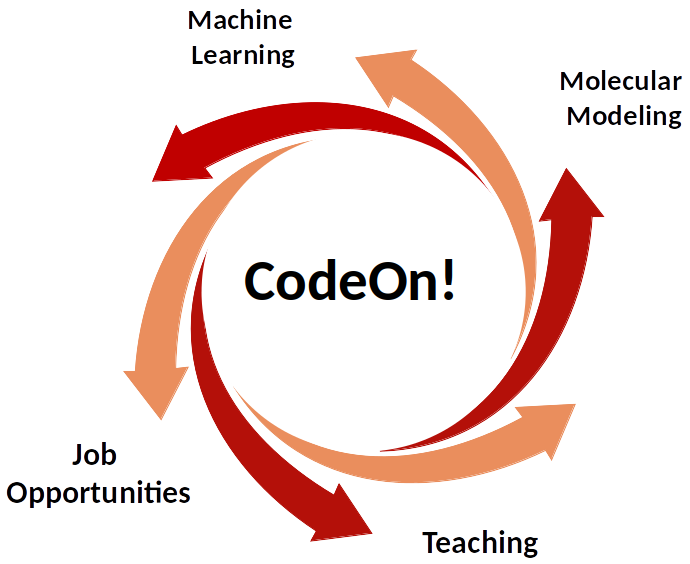
\includegraphics[width=9.58in]{~/keckcodeon/keckcodeon_blog/static/images/code_on_wheel} \end{center}


\end{document}
